\begin{figure*}
  \centering
  \begin{subfigure}[b]{\textwidth}
    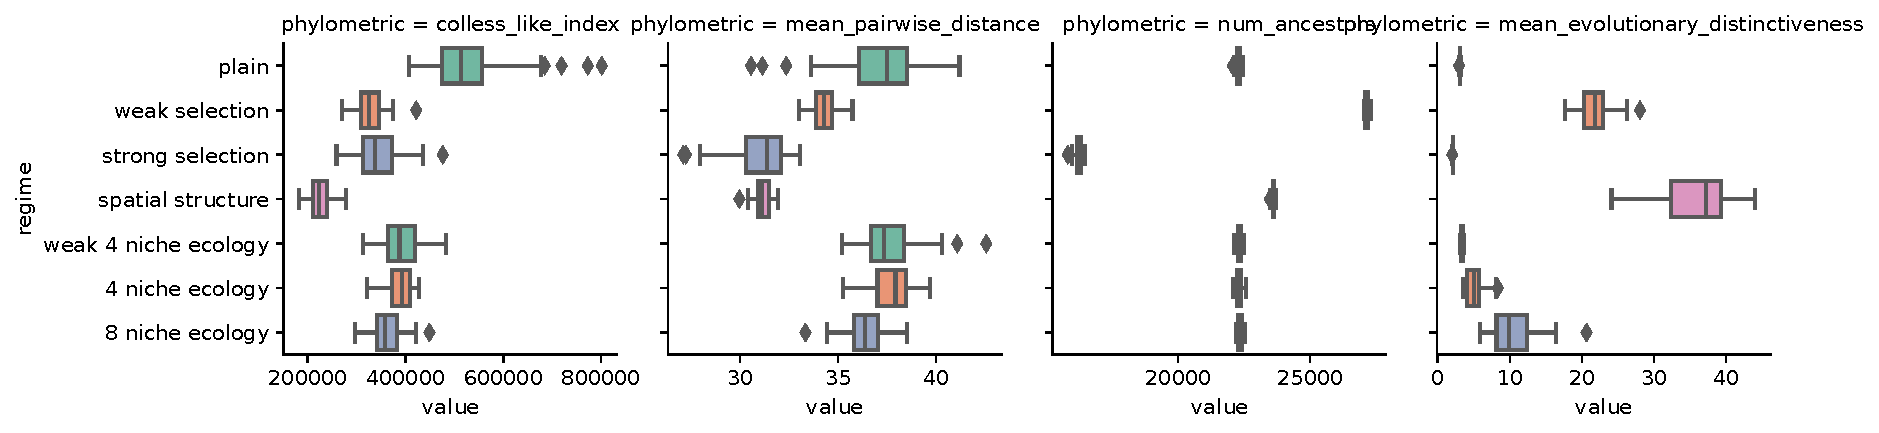
\includegraphics[width=\textwidth]{binder/binder/teeplots/col=phylometric+epoch=7+mut_distn=np.random.standard_normal+viz=boxplot+x=value+y=regime+ext=.pdf}
  \caption{%
    Distribution of phylometrics under the simple model.
    Sample sizes $n=50$.
  }
  \label{fig:perfect-tree-phylometrics-simple-boxplot}
  \end{subfigure}

  \begin{subfigure}[b]{\textwidth}
    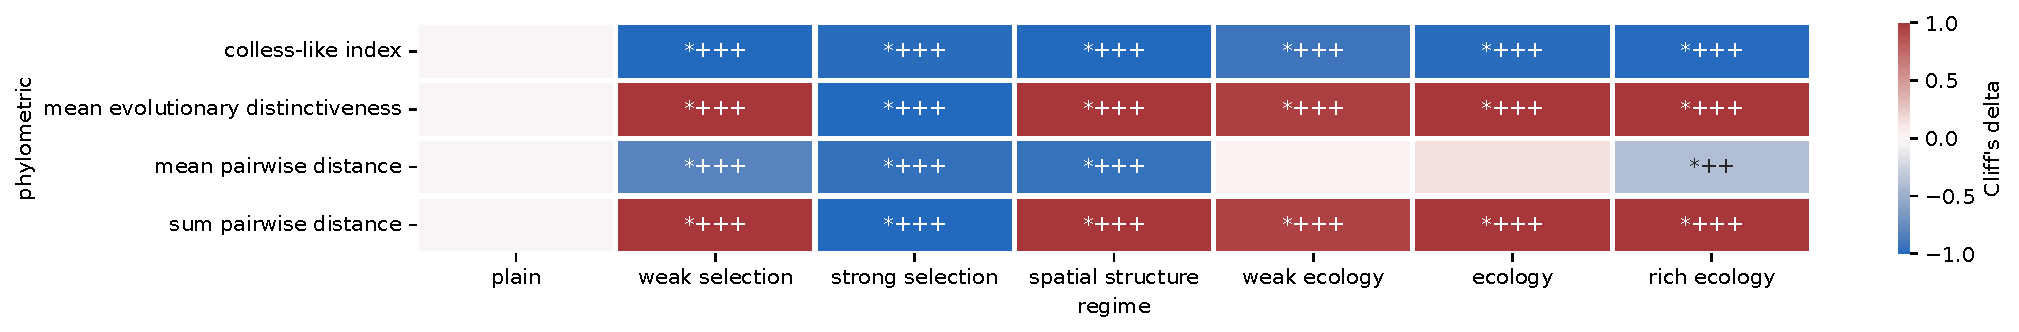
\includegraphics[width=\textwidth]{binder/binder/teeplots/epoch=7+mut_distn=np.random.standard_normal+viz=heatmap+x=regime+y=phylometric+ext=.pdf}
    \caption{
 Sizes of the effect of evolutionary regimes on each phylometric relative to ``plain'' baseline in the simple model.
    Sample sizes $n=50$.
    }
\label{fig:perfect-tree-phylometrics-simple-heatmap}
  \end{subfigure}%

\begin{subfigure}[b]{\textwidth}
  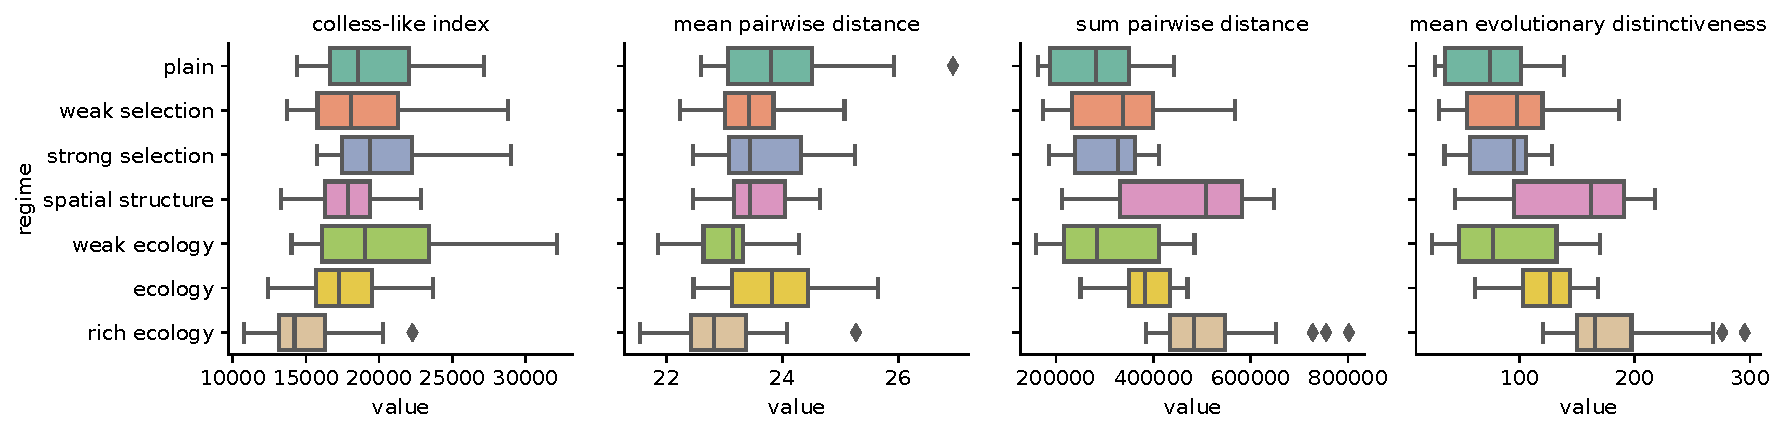
\includegraphics[width=\textwidth]{binder/binder/avida-individual/teeplots/col=phylometric+epoch=0+mut_distn=default+viz=boxplot+x=value+y=regime+ext=.pdf}
  \caption{
  Distribution of phylometrics in Avida.
  Sample sizes $n=30$.
  }
  \label{fig:perfect-tree-phylometrics-avida-boxplot}
\end{subfigure}%

\begin{subfigure}[b]{\textwidth}
  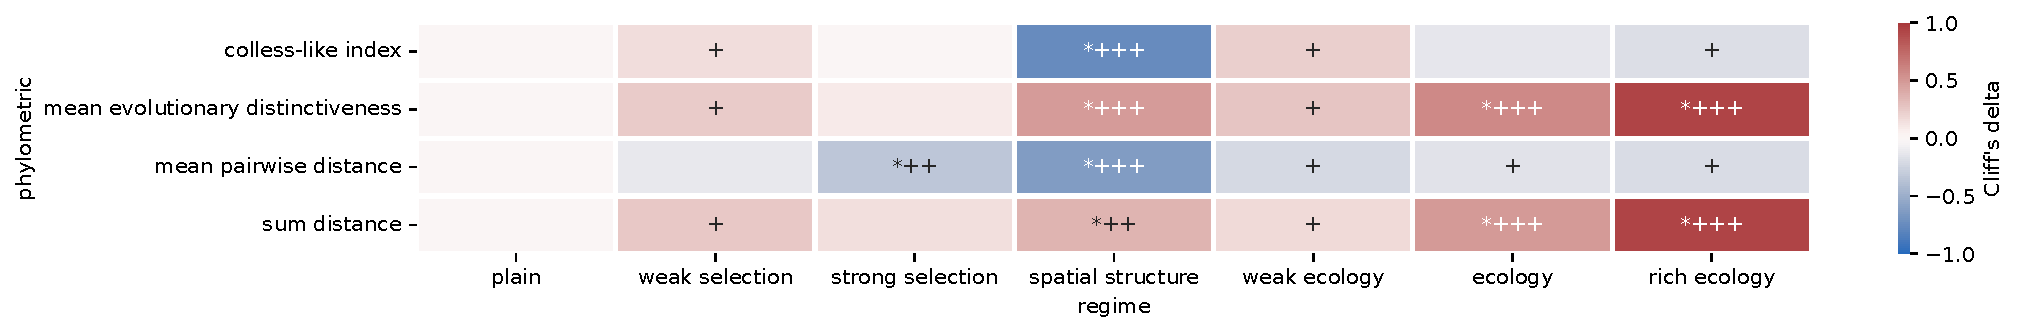
\includegraphics[width=\textwidth]{binder/binder/avida-individual/teeplots/epoch=0+mut_distn=default+viz=heatmap+x=regime+y=phylometric+ext=.pdf}
\caption{%
   Sizes of the effect of evolutionary regimes on each phylometric relative to ``plain'' baseline in Avida. Sample sizes $n=30$.
}
\label{fig:perfect-tree-phylometrics-avida-heatmap}
\end{subfigure}

  \caption{%
  \textbf{Phylometric responses for simple model and Avida.}
  Phylometrics across surveyed evolutionary regimes, calculated on perfect-fidelity individual-level phylogenies from the simple model and Avida.
  Note that nonparametric effect size normalization caps out to 1.0/-1.0 past the point of complete disbributional nonoverlap.
  For heatmap charts, +'s indicate small, medium, and large effect sizes using the Cliff's delta statistic and *'s indicate statistical significance at $\alpha = 0.05$ via Mann-Whitney U test.
  Results from simple model are for standard experimental conditions: gaussian mutation distribution at epoch 7 (generation 262,144).
  See Figure \ref{fig:perfect-tree-phylometrics-sensitivity-analysis} for results under sensitivity analysis conditions.
  }
  \label{fig:perfect-tree-phylometrics}
\end{figure*}